% %%%%%%%%%%%%%%%%%%%%%%%%%%%%%%%%%%%%%%%%%%%%%%%%%%%%%%%%%%%%%%%%%%%%%%%%%%%%
\chapter{Discovering dialogue slots}%
\label{chap:data_analysis}
% %%%%%%%%%%%%%%%%%%%%%%%%%%%%%%%%%%%%%%%%%%%%%%%%%%%%%%%%%%%%%%%%%%%%%%%%%%%%
Getting raw, unlabeled data for dialogue system training is not difficult, especially if we restrict the target domain.
In general, recording conversations in real life or artificial conditions is sufficient.
A requirement for dialogue state labels, which we discuss in Section~\ref{02:ds-background} makes this process much more costly.
The sets of slots and their values typically must be designed by domain experts.
This procedure consists of multiple tasks:
\begin{enumerate}
    \item Determine which concepts need to be captured.
    \item Define them in a consistent way.
    \item Label the occurrences of these concepts in the training data.
\end{enumerate}
As mentioned, these steps require expert knowledge and sometimes non-trivial domain understanding.
Although we might design a system that does not rely on the usage of slots, both traditional pipeline systems \cite{young_pomdp-based_2013} and end-to-end task-oriented architectures \cite{wen2016network} typically require such annotation.
While some systems presented in Section~\ref{relwork:modular} use implicit, latent state representation and do not require explicit labels, the behavior of such systems is hard to interpret or control, which can be crucial in practical applications.
Moreover, slots enable communication with external interfaces, as discussed in~\ref{02:ds-background}.
Several works are aiming at keeping interpretability and reducing the annotation needs by automating it \citep{chen2014leveraging,chen2015jointly} or transferring annotation across domains \cite{zhao_zero-shot_2018,coope_span-convert_2020}, but they still require significant manual effort.
We present a novel approach to discovering a set of domain-relevant dialogue slots and their values given a set of dialogues in the target domain (such as transcripts from a call center).
Our approach requires no manual annotation to tag slots in dialogue data.
This substantially simplifies the dialogue system design and training process, as the developer no longer needs to design a set of slots and annotate their occurrences in training data.
The content of this Chapter was published at ACL 2021~\cite{hudecek-etal-2021-discovering}.
We also present extensions to the published content to address the requirement of 3rd party models and put our method in the context of instruction-tuned LLMs.
These extensions are discussed in Section~\ref{04:sec:candidate_selection}.

\section{Method overview}
\label{04:sec:overview}
\begin{figure}[h]
    \centering
    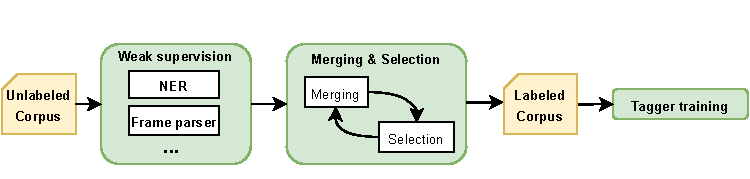
\includegraphics[width=0.9\textwidth]{images/weakly-supervised.pdf}
    \caption{Illustration of our pipeline. First, we analyze an unlabeled in-domain corpus with supplied domain-agnostic linguistic annotation models, such as a frame-semantic parser or NER. This results in slot candidates. Next, we iteratively merge and select slot candidates to obtain domain-relevant slots. Finally, we use the resulting slot labels in the corpus to train a neural slot tagger.}
    \label{fig:discover_overall}
\end{figure}
Figure \ref{fig:discover_overall} depicts a diagram describing our approach.
Our slot discovery method has three main stages:
\begin{enumerate}
    \item We obtain weak supervision labels from automatic generic annotation.
    We obtain this annotation using domain-independent natural language taggers such as a semantic frame parser or a named entity recognizer (NER).
    These models can detect important and relevant concepts in natural language utterances and subsequently group them using a set of pre-determined generic labels.
    Nevertheless, the raw output of these models is not polished and cannot be used for the purpose of the dialogue system directly.
    For more details, see Section~\ref{04:sec:tagging_concepts}.
    \item We identify domain-relevant slots based on the annotation labels by iteratively (a) merging and (b) ranking and selecting the most viable candidates (Section~\ref{04:sec:candidate_selection}).
    
    \item We use the discovered slots to train an independent slot tagger (Section~\ref{04:sec:training_tagger}).
\end{enumerate}

We refer to this approach as "weak supervision" because it uses noisy labels as input instead of the desired ones.

Consider an example in Figure \ref{fig:tagged_example}.
First, we note that it helps to use multiple tagging models since a respective model might not capture some of the concepts.
The set of tagged words from all the sources covers all the dialogue slot values (\emph{cheap}, \emph{Georgetown}).
However, it contains irrelevant words (\emph{restaurant}).
This behavior is expected since the tagging models are trained on generic open-domain data and detect all semantic concepts mentioned in the utterances.

Therefore, to exploit the output of generic models, we need to polish and customize it to the specific domain.
Our method combines multiple sources of semantic labels and selects only relevant slot candidates.
Slots discovered by our approach can then be used to design a schema relevant to a specific domain.
\begin{figure}[h]
\centering
    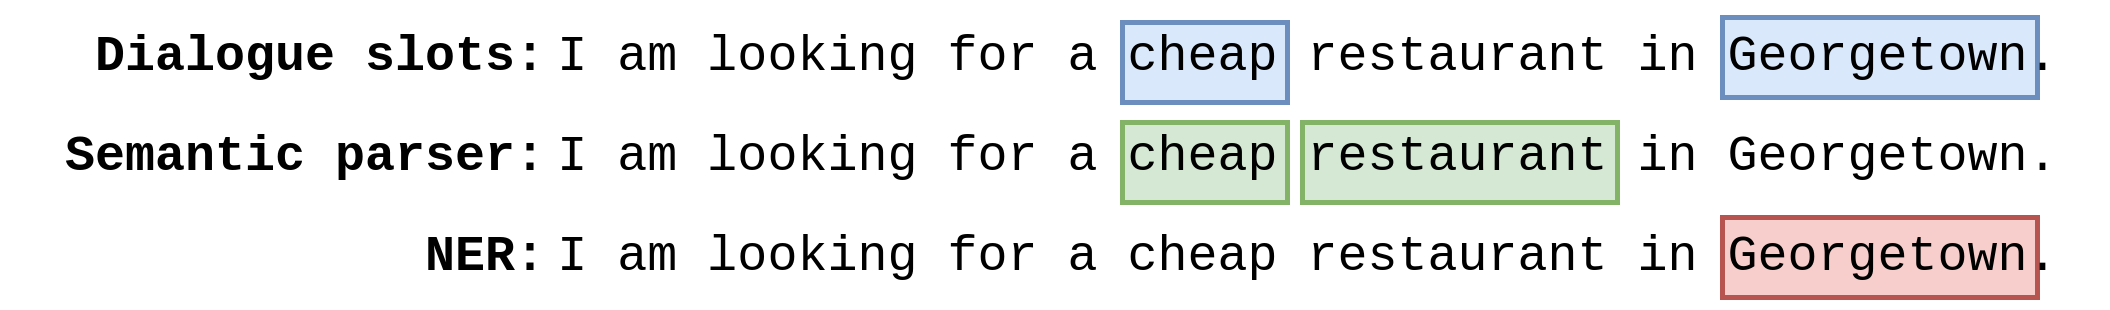
\includegraphics[width=0.8\textwidth]{images/tagging-example.png}
    \caption{An utterance from the restaurant recommendation domain tagged with generic semantic parser (green) and Named Entity Recognition system (red). We provide a comparison with ground truth dialogue slot labels (blue).}
    \label{fig:tagged_example}
\end{figure}

\section{Slot candidate identification by tagging semantic concepts}
\label{04:sec:tagging_concepts}

Our approach to selecting candidates for our method requires an initial pool of carefully chosen options representing coherent concepts. This step is critical to ensure the effectiveness of our selection process. We strive to gather as many candidates as possible to achieve this goal while preserving the above constraint.
One of the key features of our method is its ability to merge several concepts into one, which means that we aim for high granularity and specificity in our input labels. As a result, we need to ensure that each candidate represents a unique, distinguishable concept.

Given that we cannot rely on human annotations, we use an automatic procedure to gather the initial set of candidates.
This procedure combines multiple sequence tagging models to label the input corpus.
This procedure aims to identify words or phrases in the text representing distinct concepts that can be used as candidate labels.
We can use any sequence tagging NLP model that meets the following criteria: (1) a set of words with the same label indicates semantically coherent, distinct concepts, (2) no additional annotation is needed, and (3) the model is domain-independent.

For our experiments, we chose two types of taggers to obtain the input tags: Frame Semantic Parser and Named Entity Recognition (NER).
We can quickly and accurately identify candidate labels that meet our criteria by leveraging these models.


.
\begin{figure}[h!]
\centering
    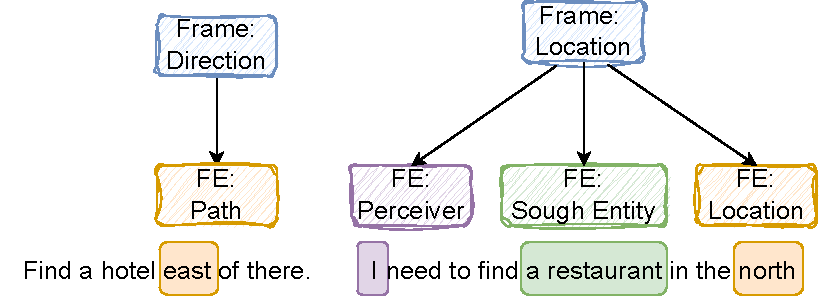
\includegraphics[width=0.8\textwidth]{images/framenet.pdf}
    \caption{An example of two Frames defined in the FrameNet dataset, together with core Frame Elements and respective instances. In this example, we can see that a semantic concept representing the location of some place can be captured by multiple frames (\emph{Direction} and \emph{Location}). However, from the perspective of dialogue systems, these differences are negligible. Therefore, we merge some of the candidates to obtain a simpler schema.}
    \label{fig:framenet}
\end{figure}

\paragraph{Frame Semantic Parser} The parser is based on the FrameNet project \cite{baker1998berkeley}.
FrameNet is a lexical database of the English language (although similar datasets exist in other languages) that aims to represent the usage of words in actual texts.
It contains over 200,000 utterances with over 1,200 frames, each representing one semantic concept.
From the NLP perspective, it can be approached as a task of Semantic Role Labeling.
Each frame is formed by one or more frame elements, which together form an instance of a certain semantic situation (e.g., \emph{Locale}, \emph{Offenses}, \emph{Size},...).
See Figure \ref{fig:framenet} for the example of FrameNet instances.
We take the individual Frame Elements as a source for our slot candidates.

\paragraph{Named Entity Recognition (NER)} is a well-established task of labeling occurrences of certain named entities in the input text data.
Typically, the NER labels \textit{word spans} that belong to a particular entity in the annotated utterance.
A common approach to identify the spans is BIO tagging \cite{ramshaw-marcus-1995-text}.
See the example in Table~\ref{04:tab:ner_example}.
\begin{table}[tp]
    \centering
    \begin{tabular}{c|c|c|c|c|c|c}
    \toprule
        \texttt{I} & \texttt{want} & \texttt{to} & \texttt{leave} & \texttt{from} & \texttt{{\color{cyan!80!yellow!80!black!100 }Edinburgh }} & \texttt{{\color{cyan!80!yellow!80!black!100 }Waverley}}. \\
        \textbf{O} & \textbf{O} & \textbf{O} & \textbf{O} & \textbf{O} & \textbf{B} & \textbf{I}\\
    \bottomrule
    \end{tabular}
    \caption{An example of BIO tagging to identify named entities.}
    \label{04:tab:ner_example}
\end{table}
It fits our requirements well because the task is universal, and the named entities definition is not specific to any particular domain.

\section{Unsupervised candidate identification}
\label{04:sec:unsup_candidate_selection}
The approach introduced in this chapter is limited by the requirement of third-party models to gather the initial set of candidates.
Therefore, we experiment with alternative ways of obtaining slot candidates completely unsupervised.
This can lift the requirement of using generic models fine-tuned on out-of-distribution data.

\subsection{Memory Networks for candidates identification}
\label{04:sec:memnn}
The end-to-end Memory Networks architecture described in Chapter~\ref{02:sec:mem_nn} suits our needs for an unsupervised slot candidate identification.
We train the Mem2Seq (see Sec.~\ref{02:sec:mem2seq}) model on the target dataset to learn the copy behavior.
We then use the trained model to obtain a set of slot candidates.
To achieve this, we let the model generate the test dialogues individually and inspect its behavior.

The Mem2Seq model's knowledge base entries represent entities or their properties, such as addresses.
Furthermore, the model saves the conversation context via the memory mechanism.
The content of the memory is further used to copy its entries directly to the produced response.
Specifically, during the response generation process, the model decides whether the new token will be generated from decoder vocabulary distribution or copied from memory.
The intuition is that when a certain token should appear in the generated response, the model decides to copy it rather than generate it to prevent mistakes.
We save each token that is copied into the produced response rather than generated.
These tokens will likely be slot candidates as they supposedly correspond to entities and slot values mentioned in the context.
We then run k-means clustering to obtain a set of slot candidates.
This way, we obtain multiple groups of word forms that can be used as input for our slot discovery pipeline.

We also note the similarity of this approach to the two-step generation process used in multiple architectures~\citep{lei2018sequicity, peng2021soloist}.
In the first step of this process, the model generates placeholders such as \emph{[address]} instead of specific values.
This delexicalized utterance is then lexicalized in the second step by replacing the placeholders with actual values, e.g. using the database.
This is almost exactly what happens in the Mem2Seq model.
Only the two steps are joined in one, so the model puts the database values indirectly.
Also, the lexicalization procedure of placing values instead of placeholders is learned rather than hardcoded.

\subsection{LLMs for candidate identification}
\begin{table}[tp]
    \centering
    \begin{tabular}{r|l}
    \toprule
        \textbf{Prompt} & \texttt{{\color{cyan!80!yellow!80!black!100 }Extract important concepts or objects }}\\
        & \texttt{{\color{cyan!80!yellow!80!black!100 }from the following utterance. }} \\
        & \texttt{{\color{cyan!80!yellow!80!black!100 } Yield all the concepts in one-level JSON dictionary. }} \\
        & \texttt{{\color{cyan!80!yellow!80!black!100 } Include only entities and concepts that}} \\
        & \texttt{{\color{cyan!80!yellow!80!black!100 } are mentioned in the utterance.}} \\
        & \texttt{{\color{cyan!80!yellow!80!black!100 } Don't provide the intent.}} \\
        & \texttt{{\color{cyan!80!yellow!80!black!100 } See the following examples:}} \\
        & \texttt{{\color{orange!50!yellow!90!black!100!} ---------- Example ------}} \\
        & \texttt{{\color{orange!50!yellow!90!black!100!} Utterance: "I am looking for a theater }} \\
        & \texttt{{\color{orange!50!yellow!90!black!100!} that is reasonably priced." }} \\
        & \texttt{{\color{orange!50!yellow!90!black!100!} Output: \{'venue': 'theater', 'price': 'reasonable'\} }} \\
        & \texttt{{\color{orange!50!yellow!90!black!100!} -------------------------}} \\
        & \texttt{{\color{cyan!80!yellow!80!black!100 } Now complete the following example: }} \\
        & \texttt{{\color{cyan!80!yellow!80!black!100 } Utterance:}  {\color{red!100!yellow!90!black!100!}"I am looking for a cheap hotel."}} \\
        & \texttt{{\color{cyan!80!yellow!80!black!100 } Output:  }} \\
        \bottomrule
    \end{tabular}
    \caption{The {\color{cyan!80!yellow!80!black!100 }prompt}, which is used to obtain slot candidates from the input utterance. It contains an {\color{orange!50!yellow!90!black!100!} example} to specify the desired output structure }
    \label{04:tab:prompt}
\end{table}

Another way of obtaining the slot candidates is by employing Large Language Models.
These models can be instructed in the input text (prompted) to perform virtually any task (see Section~\ref{background:plms}).
In our case, we instruct the model to extract the potential slot candidates directly from the input utterance.
We use two models: \emph{Tk-Instruct-11B} \cite{supernaturalinstructions}, which is T5 encoder-decoder architecture \cite{2020t5} tuned on a dataset of over 5M task instances with instructions and \emph{ChatGPT} which is a closed source product introduced by the OpenAI company\footnote{\url{https://openai.com/blog/chatgpt}}.
The used prompt is given in Table~\ref{04:tab:prompt}.
We use both models in parallel to obtain two sets of candidates.
We then use a clustering procedure similar to the process described in~\ref{04:sec:memnn}.
Note that although the model categorizes the extracted words as part of the output, the category names are arbitrary and inconsistent among examples.
For example, the model can categorize a word \emph{Italian} once as \textit{food\_type} and on another occasion as \emph{nationality}.
Therefore, we do not use them to obtain the slot groups directly.
This leaves us with a set of slot candidates again used as input to our pipelined method.

\section{Selection of slot candidates}
\label{04:sec:candidate_selection}
% \begin{figure}[ht]
%     \centering
%     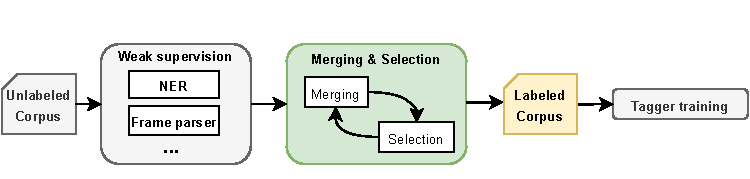
\includegraphics[width=0.9\textwidth]{images/merging.pdf}
%     \caption{The selection step in our pipeline processes the input data and yields a set of slot candidates that should be relevant to the target domain.}
%     \label{fig:candidate_selection}
% \end{figure}
In the previous step, we obtained a superset of all the slot candidates using weak supervision from the tagging models.
Subsequently, we need to identify domain-relevant slots based on candidates provided by the automatic annotation.
To achieve this, we design an iterative slot discovery procedure -- in each iteration, we: 
(1) merge similar candidates, 
(2) rank candidates' relevance and eliminate irrelevant ones.
Once no more frames are eliminated, the process stops and we obtain slot labels, which are used to train a slot tagger (see Section~\ref{04:sec:training_tagger}).

We refer to the automatically tagged tokens as \emph{(slot) fillers}, and the tags are considered slot candidates.
To be able to select relevant candidates, we need to represent them in continuous space.
We use word embedding vectors and compute \emph{slot embeddings} $e(s_k)$ for each 
distinct slot candidate $s_k$ as word embedding averages over all respective slot fillers, weighted proportionally by filler frequency.
The merging step requires the slot embeddings to be re-computed after each iteration.
We will now describe the individual steps.

\subsection{Candidate Merging}
\label{03:candidate_merging}
Since automatic annotation may have a very fine granularity, multiple slot candidates often capture entities/objects of the same type.
This is the case for frame-semantic annotation, which we mostly use in our experiments.
With a frame parser, for instance, the frames \emph{Direction} and \emph{Location} both relate to the concept of \emph{area}, which can be represented as a single slot.
Thus, we must merge similar slot candidates subsets $s_1 \dots s_n$ under a single candidate.
We further use a syntactic parser to obtain dependency relations in which the slot fillers appear in the data and use this information to get more accurate similarity scores.
We measure the similarity of slot candidates $s_1,s_2$ as:
\begin{equation}
    \text{sim}(s_1,s_2) = \text{sim}_{e}(e(s_1),e(s_2)) + \text{sim}_{\text{ctx}}(s_1,s_2)
\end{equation}
where $\text{sim}_{e}$ is a cosine similarity and $\text{sim}_{\text{ctx}}(s_1,s_2)$ is a normalized number of occurrences of $s_1$ and $s_2$ with the same dependency relation.
If the similarity exceeds a pre-set threshold $T_{\text{sim}}$, the candidates are merged into one.

\subsection{Candidate Ranking and Selection}
\label{04:candidate_select}
In this step, we aim to eliminate irrelevant slot candidates and exclude them from the selection process.
To achieve this, we rank the slot candidates with respect to their importance computed from the data.
We hypothesize that different slots are likely to occur in different contexts (e.g., addresses are mentioned more when the system provides information to the user rather than stated by the user).
Some slots can occur rarely but still be relevant.
However, such rare slots would be overshadowed by more frequent slot candidates.
To preserve relevant slots that only occur in rarer contexts, we cluster the data into multiple clusters and then rank the candidates within each cluster separately.
Finally, we filter the candidates according to a threshold.
Specifically, we consider all candidates with a score higher than the chosen threshold relevant and select them for the next iterations.
The threshold is determined as an $\alpha$-fraction of a given cluster mean where $\alpha$ is chosen empirically.
If a slot candidate is selected in at least one of the clusters, it is considered viable overall.

\paragraph{Clustering the data}
The data clustering step aims to distinguish contexts in which the candidates appear.
We simplify the notion of context to the head verb connected with the respective slot filler word.
We process the data with a generic semantic role labeling tagger to obtain verb dependency relations.
Each occurrence of a filler is thus associated with a \emph{head verb} whose semantic argument the corresponding word is, if such exists. 
To give an example, consider \emph{verb-filler} pairs such as \emph{want-chinese} or \emph{reserve-hotel}.
We then compute embeddings of the formed pairs.
To do this, we take an embedding of both the head verb and the fillers and average them.
The pairs are then clustered using agglomerative (bottom-up) hierarchical clustering with average linkage according to the cosine distance of their embeddings.
Note that fillers for the same slot candidate may end up in multiple clusters.
This does not mean that the respective slot candidate is split -- it is just ranked for relevance multiple times (with respect to multiple contexts).
The process stops when a predetermined number of clusters is reached.

\paragraph{Candidate Ranking criteria}
We need a function that computes a score for each candidate to rank the candidates.
Since it is unclear how to compute the score, we combine multiple attributes to compute the final score.
Specifically, we compute the following characteristics for each candidate:
\begin{itemize}
    \item \textbf{Frequency} $\text{frq}(s)$ is used since candidates that occur frequently in the data are likely important.
    
    \item \textbf{Coherence} $\text{coh}(s)$ is the average pairwise similarity of all fillers' embeddings:
    \begin{equation}
        \text{coh}(s) = \frac{\mathlarger{\sum}_{(v,w) \in C^2_s}{d_{\cos}(e(v), e(w))}}{|C^2_s|}
    \end{equation}
    where $C^2_s$ is a set of all pairs of fillers for the slot candidate \emph{s}.
    We follow \citet{chen2014leveraging}'s assumption that fillers with high coherence, i.e., focused on one topic, are good slot candidates.
    
    \item \textbf{TextRank} \cite{mihalcea2004textrank} is a keyword extraction algorithm similar to the well-known PageRank~\citep{page1999pagerank}.
    It constructs a graph where nodes represent words and edges represent their co-occurrence.
    The dominant eigenvector of the adjacency matrix of this graph then gives the individual words' scores.
\end{itemize}
The final score is a simple sum of rankings with respect to all three scores.
For TextRank and frequency, we use a placeholder representing the slot candidate instead of the respective fillers.
Therefore, we obtain scores relevant to candidates rather than the individual words.

\section{Training standalone tagger}
\label{04:sec:training_tagger}
% \begin{figure}[h]
%     \centering
%     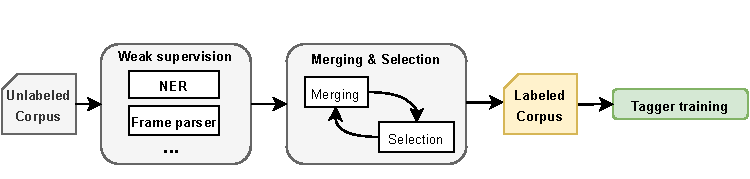
\includegraphics[width=0.9\textwidth]{images/tagging.pdf}
%     \caption{After the set of slots is selected we assign the obtained labels to their occurrences in the data and use this labeled corpus to train a standalone tagger. }
%     \label{fig:training_tagger}
% \end{figure}
The steps described in Sections~\ref{04:sec:tagging_concepts}, \ref{04:sec:unsup_candidate_selection} and \ref{04:sec:candidate_selection} can give us a good set of dialogue slots. % to be tracked.
However, directly using the merged and filtered slots may result in low recall since the original annotation models used as weak supervision are not adapted to our specific domain.
Therefore, we use the obtained labels to train a new, domain-specific slot tagger to improve performance.
The tagger has no access to better labels than those derived by our method; however, it has a simpler task, as the set of target labels is now much smaller, and the domain is much narrower.

The motivation for training a tagger is two-fold.
First, its usage makes it possible to discard a dependency on the candidate identification models in runtime.
Thus, the method is simpler to apply. 
Second, although the selection process can yield a good set of slot candidates, we experimentally discovered that the quality of the taggers used for initial input labeling can be insufficient, especially for some domains.
Therefore, directly using the merged and filtered slots may result in low recall since the original annotation models used as weak supervision are not adapted to our specific domain.

We model the slot tagging task as sequence tagging, using a convolutional neural network that takes word- and character-based embeddings of the tokens as the input and produces a sequence of respective tags \cite{lample2016neural}.\footnote{\url{https://github.com/deepmipt/ner}}
The output layer of the tagger network gives softmax probability distributions over possible tags.

\paragraph{Increasing recall} To further increase recall, we add an inference-time rule -- if the most probable predicted tag is `O' (i.e., no slot) and the second most probable tag has a probability higher than a preset threshold $T_{\text{tag}}$, the second tag is chosen as a prediction instead.
As we discuss in Section \ref{04:sec:discovery_results}, this threshold is crucial for achieving substantial recall improvement.

\paragraph{Tagging model robustness} 
We only use 10\% of the original in-domain training set (with labels from Section~\ref{04:sec:tagging_concepts}) to train the slot tagger model.
The rest of the training set is used for a grid search to determine model hyperparameters (hidden layer size, dropout rate, and $T_{\text{tag}}$ threshold). We choose the parameters that yield the best F1 score when compared against the automatic slot discovery results (i.e., no manual annotation is needed here; the aim is a good generalization and improved robustness of the resulting model).


\section{Experimental setup}
\label{04:sec:discovery_results}
In this section, we provide a quantitative analysis of the results with respect to the NLU performance and quality of the discovered slots.
We also evaluate the application of this method as a module in the end-to-end dialogue system model.
\paragraph{Datasets}
We use multiple datasets to evaluate the proposed method extensively and gain more insights.
The datasets vary in several properties, like domain count or collection process.
This means we can compare the results on different data distributions and tasks with different complexities.
For more detailed dataset descriptions, please refer to Section \ref{02:sec:input-data-desc}.
Here, we provide only a concise list with basic descriptions.
\begin{itemize}
    \item \textbf{CamRest676} (\textbf{CR}) is dataset of 2,744 user utterances, all in the restaurant reservation domain.
    \item \textbf{Cambridge SLU} (\textbf{CS}) is in the same domain as CamRest676 but only focuses on NLU annotation of  10,569 user utterances.
    \item \textbf{MultiWOZ} is a multi-domain dialogue corpus. For experiments in this chapter, we picked only single-domain dialogues from two domains -- hotel reservation and attraction recommendation -- to form \textbf{WOZ-hotel} (\textbf{WH}) with 14,435 utterances, 9 slots, 3 intents and \textbf{WOZ-attr} (\textbf{WA}) with 7524 utterances, 8 slots and 3 intents respectively.
    \item \textbf{ATIS} (\textbf{AT}) is focused on flight search and contains nearly 5,000 utterances.
\end{itemize}
\paragraph{3rd party models}
As sources of weak supervision providing slot candidates, we mainly use the frame semantic parsers \textit{SEMAFOR} \cite{das2010semafor} and \textit{open-sesame} \cite{swayamdipta2017frame} -- a union of labels provided by both parsers is used in all our setups. In addition, to explore combined sources on the named-entity-heavy ATIS dataset, we include a generic convolutional NER model provided by SpaCy.\footnote{\url{https://spacy.io}}
To provide features for slot candidate merging and selection, we use AllenNLP \cite{Gardner2017AllenNLP} for SRL
and FastText \cite{bojanowski2017enriching} as pre-trained word embeddings.

\subsection{Training details}
\begin{itemize}
    \item Slot merging and selection parameters were set heuristically in an initial trial run on the CamRest676 data and proved stable across domains.
    \item Slot tagger hyperparameters are chosen according to grid search on a portion of the training data.
    \item Since the models are rather small concerning the number of parameters, it is sufficient to use a regular desktop PC. In our experiments, we require about 4 GB of RAM and use Intel Xeon E5-2630 v4 CPUs. 
    \item Our slot candidate selection step takes roughly 1 hour.
    The tagger model is lightweight, with only 150k parameters. Its training requires 10-30 minutes, depending on the exact configuration and data size.
    \item We conduct a hyperparameter search using a basic grid search algorithm. We tested hidden size values $\in [50,200]$, dropout $\in [0.5,0.85]$ and the threshold $T_{\text{tag}} \in [0.05,0.3]$. Therefore, we ran $4\times8\times6 = 192$ search trials.
    \item The best parameters were determined by tagger accuracy on the validation set: hidden\_size = 250, dropout = 0.7, $T_{\text{tag}} = 0.3$, $T_{\text{sim}} = 0.9$.
    \item For data without explicit \emph{train:validation:test} splits we use ratio of sizes \emph{8:1:1}.
\end{itemize}

\subsection{Evaluated systems}
We test multiple variants of our system.
This gives us an idea about the contributions of all the individual methods we propose.
Here we give an overview of all the system variants:
\begin{itemize}[nosep,leftmargin=10pt]
    \item \textit{Ours-full} is the full version of our method (full annotation setup and trained slot tagger).
    \item \textit{Ours-nothr} does not use the recall-increasing second-candidate rule in the slot tagger.
    \item \textit{Ours-notag} excludes the slot tagger. This means that the outputs of input taggers are used directly to annotate the data.
    \item \textit{Ours-nocl} further excludes the clustering step; slot candidate ranking and selection is performed over all candidates together.
\end{itemize}
We also compare to previous work of \citet{chen2014leveraging}\footnote{We use our re-implementation of their approach.}.
This method is similar to the variant \textit{Ours-nocl} but does not merge similar frames and uses different ranking criteria.
Essentially, they use the outputs of the input tagger directly after the selection step without further processing.

To put our results into perspective, we also include two supervised models for comparison:
\emph{Tag-supervised} is the same model that we use as our slot tagger (see \ref{04:sec:training_tagger}), but it is trained on supervised data with all ground truth labels available.
The other supervised baseline is called \emph{Dict-supervised}.
It uses a simple dictionary of slot fillers obtained directly from the training data.
We use straightforward word matching based on regular expressions to tag occurrences of these values.

Apart from evaluating the tagging performance with respect to NLU, we are also interested in the intrinsic evaluation of the verb-slot pair clusters formed for slot ranking.
Specifically, we ask how well these clusters are formed and if they are meaningful.
We compare to gold-standard intent annotation with respect to the following baselines: (1) a majority baseline (assigning the most frequent intent class to all instances), and (2) a simple method that represents the utterances as averages of respective word embeddings and performs sentence-level intent clustering.
All the slots in a given utterance are assumed to have the same intent.

\begin{figure}[tp]
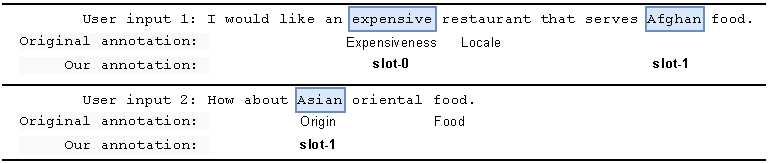
\includegraphics[width=1.0\textwidth]{images/label_example.pdf}
%\newtcbox{\bluebox}[1][]{nobeforeafter, tcbox raise base, shrink tight, sharp corners, extrude by=1mm, colback=blue!15, colframe=blue, #1}
%\newtcbox{\graybox}[1][]{nobeforeafter, tcbox raise base, shrink tight, sharp corners, extrude by=1mm, colback=gray!15, colframe=gray, #1}
%\small
%        \centering
%        \begin{tabular}{rl}
%        \hline
%        \texttt{user input 1:} & \textit{\texttt{I would like an \bluebox{expensive} \graybox{restaurant} that serves \bluebox{Afghan} food }} \\
%        \texttt{original annotation:} & \hspace{29mm} Expensiveness \hspace{4mm} Locale \hspace{33mm} - \\
        %\rowcolor{lightblue}
%        \texttt{our slot tagger:} & \bf\hspace{31mm} slot-0 \hspace{15mm} - \hspace{38mm}slot-1  \\
%        \hline
%        \texttt{user input 2:} & \textit{\texttt{How about \bluebox{Asian} oriental \graybox{food}?}} \\
%        \texttt{original annotation:} & \hspace{19mm} Origin \hspace{19mm} Food \\
        %\rowcolor{lightblue}
%        \texttt{our slot tagger:} & \bf\hspace{20mm}slot-0 \hspace{22mm} - \\
%        \hline
%        & ...
%        \end{tabular}
        \caption{A sample of a dialogue from CamRest676 data, with labels from a frame-semantic parser (middle) and our slot tagger (bottom).
        Although ``Afghan'' food is not in the frame parser output, our tagger could recognize it. The second utterance successfully captures the change in value for slot-1 (corresponding to food type). This shows that our model can categorize entities (both ``Afghan'' and ``Asian'' relate to the same slot).}
    \label{fig:example}
\end{figure}
\section{Evaluation}
We need a way of comparing the predicted structure to the ground truth to evaluate the discovered set of slots.
Therefore, we construct a handcrafted mapping between our discovered slots and the respective ground-truth slots.
Importantly, this mapping is only needed for evaluation; \textbf{our method does not depend on it}.
The mapping is domain-specific, but it is very easy to construct even for an untrained person -- the process takes less than 10 minutes for each of our domains.
It amounts to matching slots from the domain ontology against slots output by our approach, represented by the FrameNet labels.
We provide an example of such a reference mapping in Table \ref{03:ref_mapping}.
\label{sec:app-ref-mapping}

\begin{table}[tp]
    \centering
    \small
    \begin{tabular}{rcl}
    \textbf{\emph{Ours-full} output} & & \textbf{CambridgeSLU ontology}\\\hline
     Expensiveness & $ \mapsto$ & Pricerange\\
     Origin + People\_by\_origin & $ \mapsto$ & Food\\
     Direction + Part\_orientational & $ \mapsto$ & Area\\
     Contacting + Artifact & $ \mapsto$ & Phone\\
     Locale\_by\_use & $ \mapsto$ & Type \\
     

    \end{tabular}
    \caption{An example of reference mapping between the output of \emph{Ours-full} represented by FrameNet labels (left) and ground-truth CambridgeSLU ontology (right).
    Frames merged by our method are shown on a single line, separated by “+”.
    }
    \label{03:ref_mapping}
\end{table}

We use some common metrics described in Section \ref{02:sec:eval_metrics} for quantitative evaluation.
Specifically we use \textbf{Intent Accuracy}, \textbf{Joint Goal Accuracy} and \textbf{Entity Match Rate.}
We also use some metrics specific to this part of the work:
\begin{itemize}
    \item \textbf{Slot F1 score}: To reflect slot tagging performance, we measure precision, recall, and F1 for every slot individually.
    An average is then computed from slot-level scores, weighted by the number of slot occurrences in the data.
    We measure slot F1 on standalone user utterances (slot tagging) and in the context of a dialogue system (dialogue tracking).
    \item \textbf{Slot-level Average Precision (AP)}. The slot candidates picking task is a ranking problem, and we use the \textit{average precision} metric following \citet{chen2014leveraging}.
    Considering a ranked list of discovered slots $l = s_1, \dots, s_k, \dots, s_n$ we compute AP:
    \begin{equation}
        AP(l) = \frac{\sum_{k=1}^n P@k(l)\mathbbm{1}_k}{\mbox{\#\,mapped\ slots}}
    \end{equation}
    where $\mathbbm{1}_k$ is an indicator function that equals one if slot $k$ has a reference mapping defined and $P@k(l)$ is precision at $k$ of the ranked list $l$.
    \item \textbf{Slot Rand Index (RI)} is a clustering metric used to evaluate slot candidate merging. RI is the proportion of pairs of slot candidates correctly assigned to the same or different slots (following the reference mapping).\footnote{We compute RI on a union of labels with a ground-truth slot mapping and all labels selected by our method. Labels without ground-truth mapping are assumed to form single-item “pseudo-slots”.}
    
    \item \textbf{Normalized Mutual Information (NMI)} is the mutual information between two clusterings normalized into the (0, 1) interval.
    Thanks to the normalization, it is suitable for comparing two clusterings with different numbers of clusters.
\end{itemize}

For slot tagging and ranking evaluation, we sampled a random data order 50 times and performed 5-fold cross-validation for each permutation.
For the dialogue generation evaluation, we trained the models 100 times and used averaged results.
All results are given with 95\% confidence intervals.

\begin{figure}
    \centering
    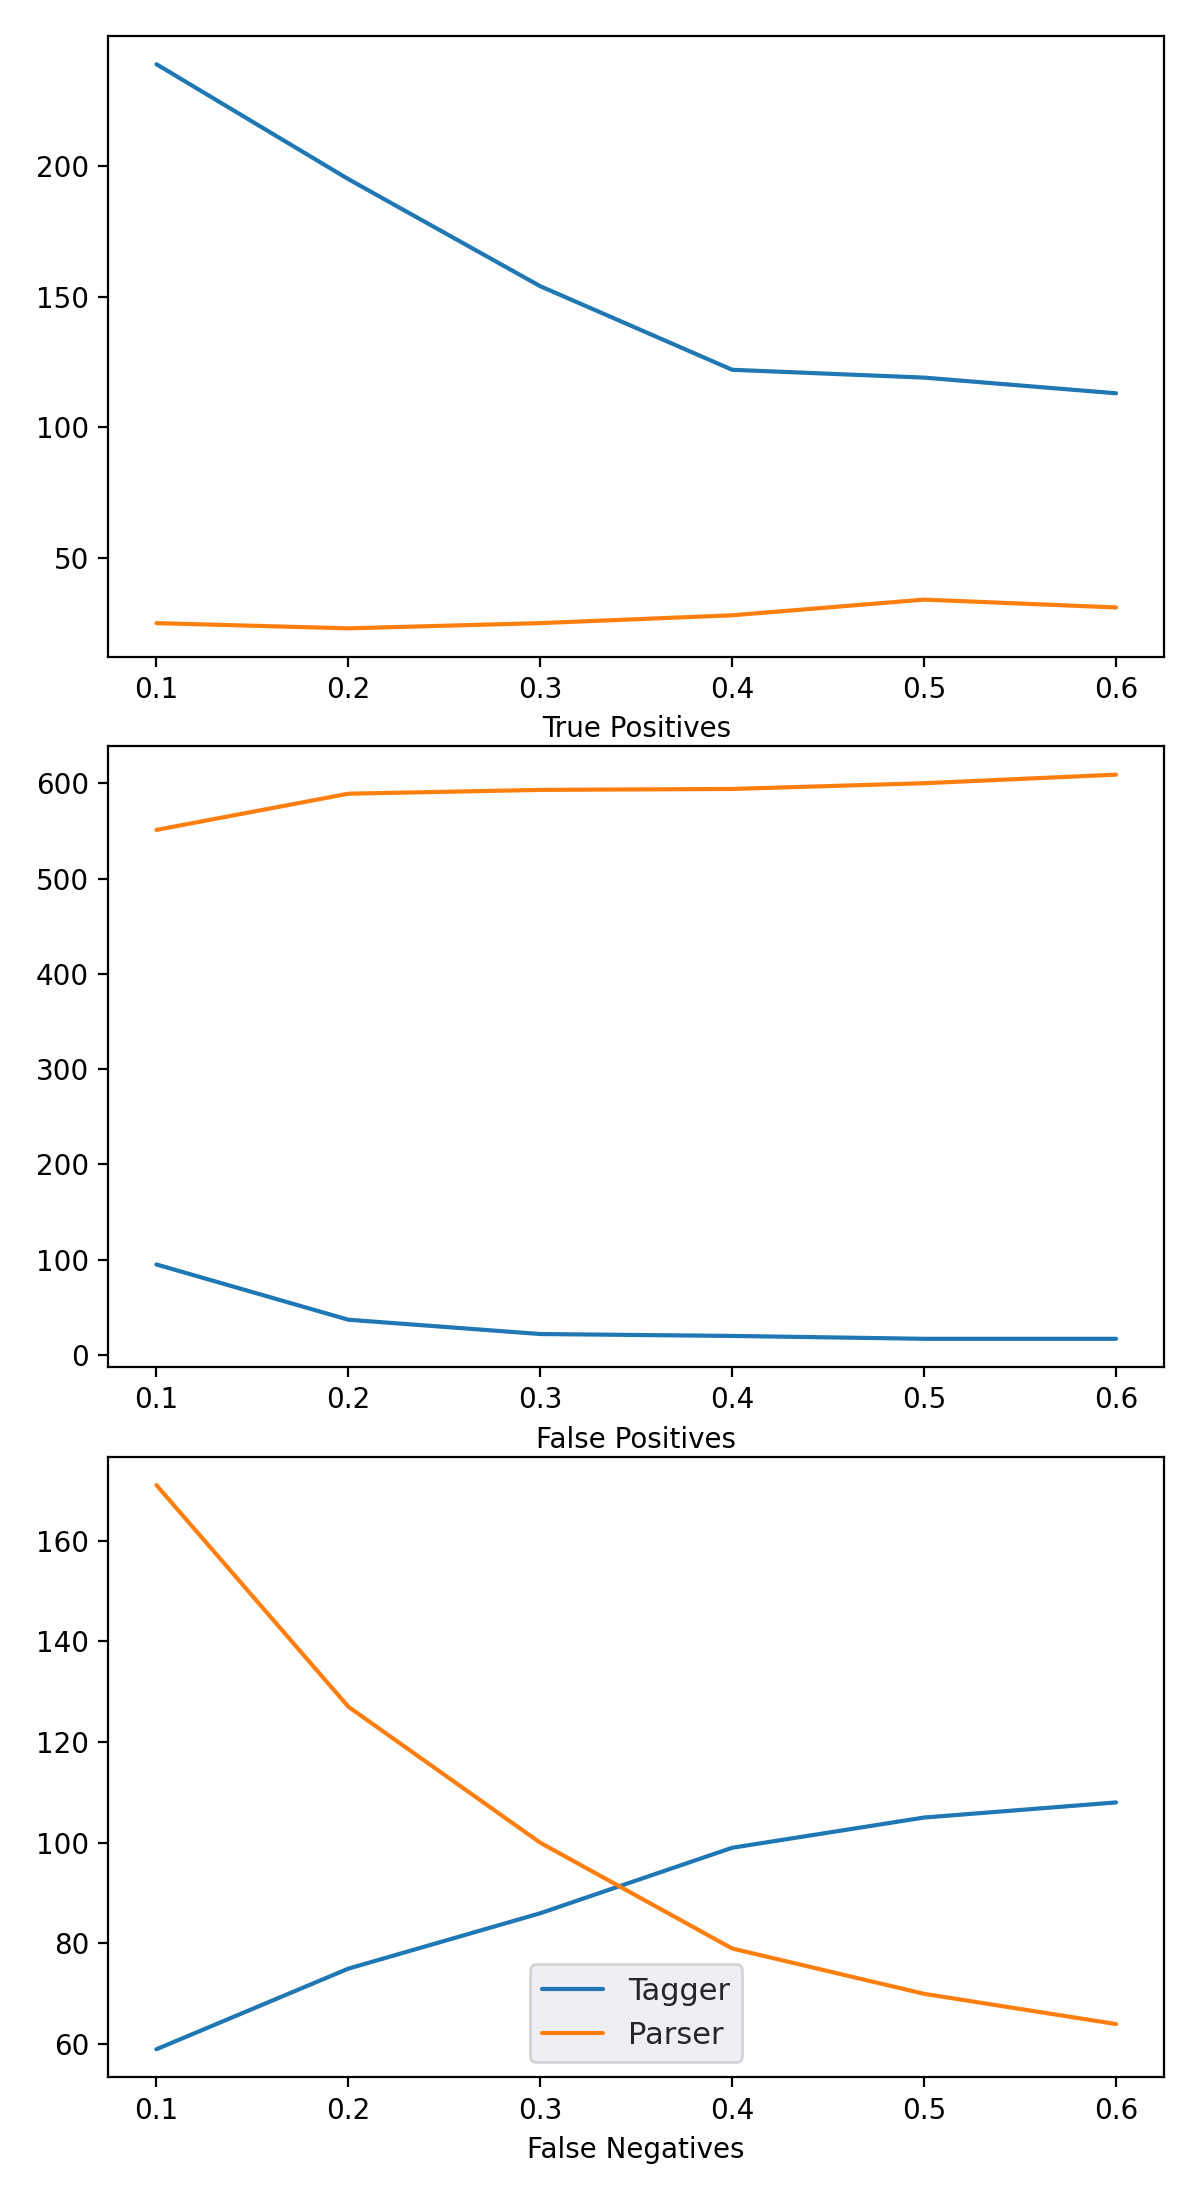
\includegraphics[width=0.6\textwidth]{images/slots.png}
    \caption{The comparison of outputs of our tagger and the parser. The plots show a number of cases in which the respective approach encounters more TPs, FPs, or FNs than the other.}
    \label{fig:tagger_comp}
\end{figure}

\section{Results}
We evaluate our approach to slot discovery by comparing the resulting slot labels to gold-standard supervised slot annotation.

\paragraph{Slot tagging}\hspace{-3mm} is evaluated in Table \ref{table:slotfilling}.
\emph{Ours-full} (slot selection + trained tagger) outperforms all other approaches by a large margin, especially regarding recall.

The performance cannot match the supervised models, but it is not far off in some domains.\footnote{Note that our measurements of slot F1 only consider the `O' tag as negative (the average is computed over slots only). This results in lower numbers than those reported in literature \cite{goo_slot-gated_2018}, but we believe this reflects the actual performance more accurately.}
\citet{chen2014leveraging}'s method has a slightly higher precision, but our recall is much higher than theirs.
Note that \citet{chen2014leveraging} do not reduce the set of candidates.
They only rank them so that a manual cut-off can be made.
In contrast, our method reduces the set of candidates significantly.
A comparison between \textit{Ours-notag} and \textit{Ours-full} shows that applying the slot tagger improves both precision and recall.
Tagger without the threshold decision rule (\textit{Ours-nothr}) mostly performs better than the parser; however, using the threshold is essential to improve recall.
Experiments on ATIS with NER as an additional annotation source proved that our method can benefit from it.
As discussed above, using the trained tagging model is crucial to improve the recall of our method. In Figure~\ref{fig:tagger_comp}, we compare the results with and without the tagger. We change the value of the prediction threshold and measure the number of cases in which the tagging model encounters more true positives, false positives, or false negatives, respectively. As the results show, lowering the threshold increases the number of cases in which the tagger finds more correct slot values (and therefore improves recall), while it does not affect the number of false positives much (and therefore retains precision).
\begin{table}[tp]
        \centering
        \small
        \begin{tabular}{l|c|c|c|c}
        \hline
         \textbf{method} $\downarrow$ / \textbf{dataset}$ \rightarrow$ &  \textbf{CS} & \textbf{WH} & \textbf{WA} & \textbf{AT} \\
         \hline
        Tag-supervised$^\ast$ & $0.724 \pm .003 $ & $\pmb{0.742} \pm .008$ & $\pmb{0.731} \pm .002$ & $\pmb{0.848} \pm .003$ \\
         Dict-supervised$^\ast$ & $\pmb{0.753} \pm .005 $ & $\pmb{0.750} \pm .018$ & $0.665 \pm .003$ & $0.678 \pm .002$ \\\hline
        \bf weak supervision $\rightarrow$ & frames & frames & frames &  frames,NER \\\hline
         Chen et al. & $0.590 \pm .001 $ & $0.382 \pm .001$ & $0.375 \pm .001$ & $0.616 \pm .001$  \\\hdashline[0.5pt/2pt]
         %\hline
         Ours-nocl & $0.393 \pm .011 $ & $0.122 \pm .001$ & $0.266 \pm .008 $ & $ 0.677 \pm .002$ \\
         %\hline
         Ours-notag & $0.664 \pm .007$ & $0.388 \pm .002$ & $0.383 \pm .002$ & $ 0.648 \pm .003$ \\
         Ours-nothr & $0.569 \pm .031$ & $0.485 \pm .032$ & $0.435 \pm .002 $ & $0.698 \pm .004$\\
         %\hline
         Ours-full & $\pmb{0.692} \pm .008$ & $\pmb{0.548} \pm .004$ & $\pmb{0.439} \pm .001$ & $\pmb{0.710} \pm .002$ \\
         \hline
        \end{tabular}
                 
        \caption{F1 score values with 95\% confidence intervals for slot tagging performance comparison among different methods. The measures are evaluated using a manual slot mapping to the datasets' annotation, which is unnecessary for the methods. $^\ast$Note that supervised setups are not directly comparable to our approach.
        \label{table:slotfilling}
        }
\end{table}

\paragraph{Performance of unsupervised candidate identification}
We separately evaluate the setup in which we used unsupervised sources of candidate identification described in Section~\ref{04:sec:unsup_candidate_selection}.
In Table~\ref{04:tab:unsup-discovery}, we present the performance of the overall pipeline for various candidate identification methods with and without applying our full pipeline (see~\ref{04:sec:overview}).
We can see that applying our pipeline improves the performance, especially the overall recall.
We also compare the pipeline performance with various candidate identification methods in Figure~\ref{04:fig:compare_sources}.
This comparison shows that the FrameNet-based candidate identification mechanism outperforms unsupervised variants.
\begin{figure}[h]
    \centering
    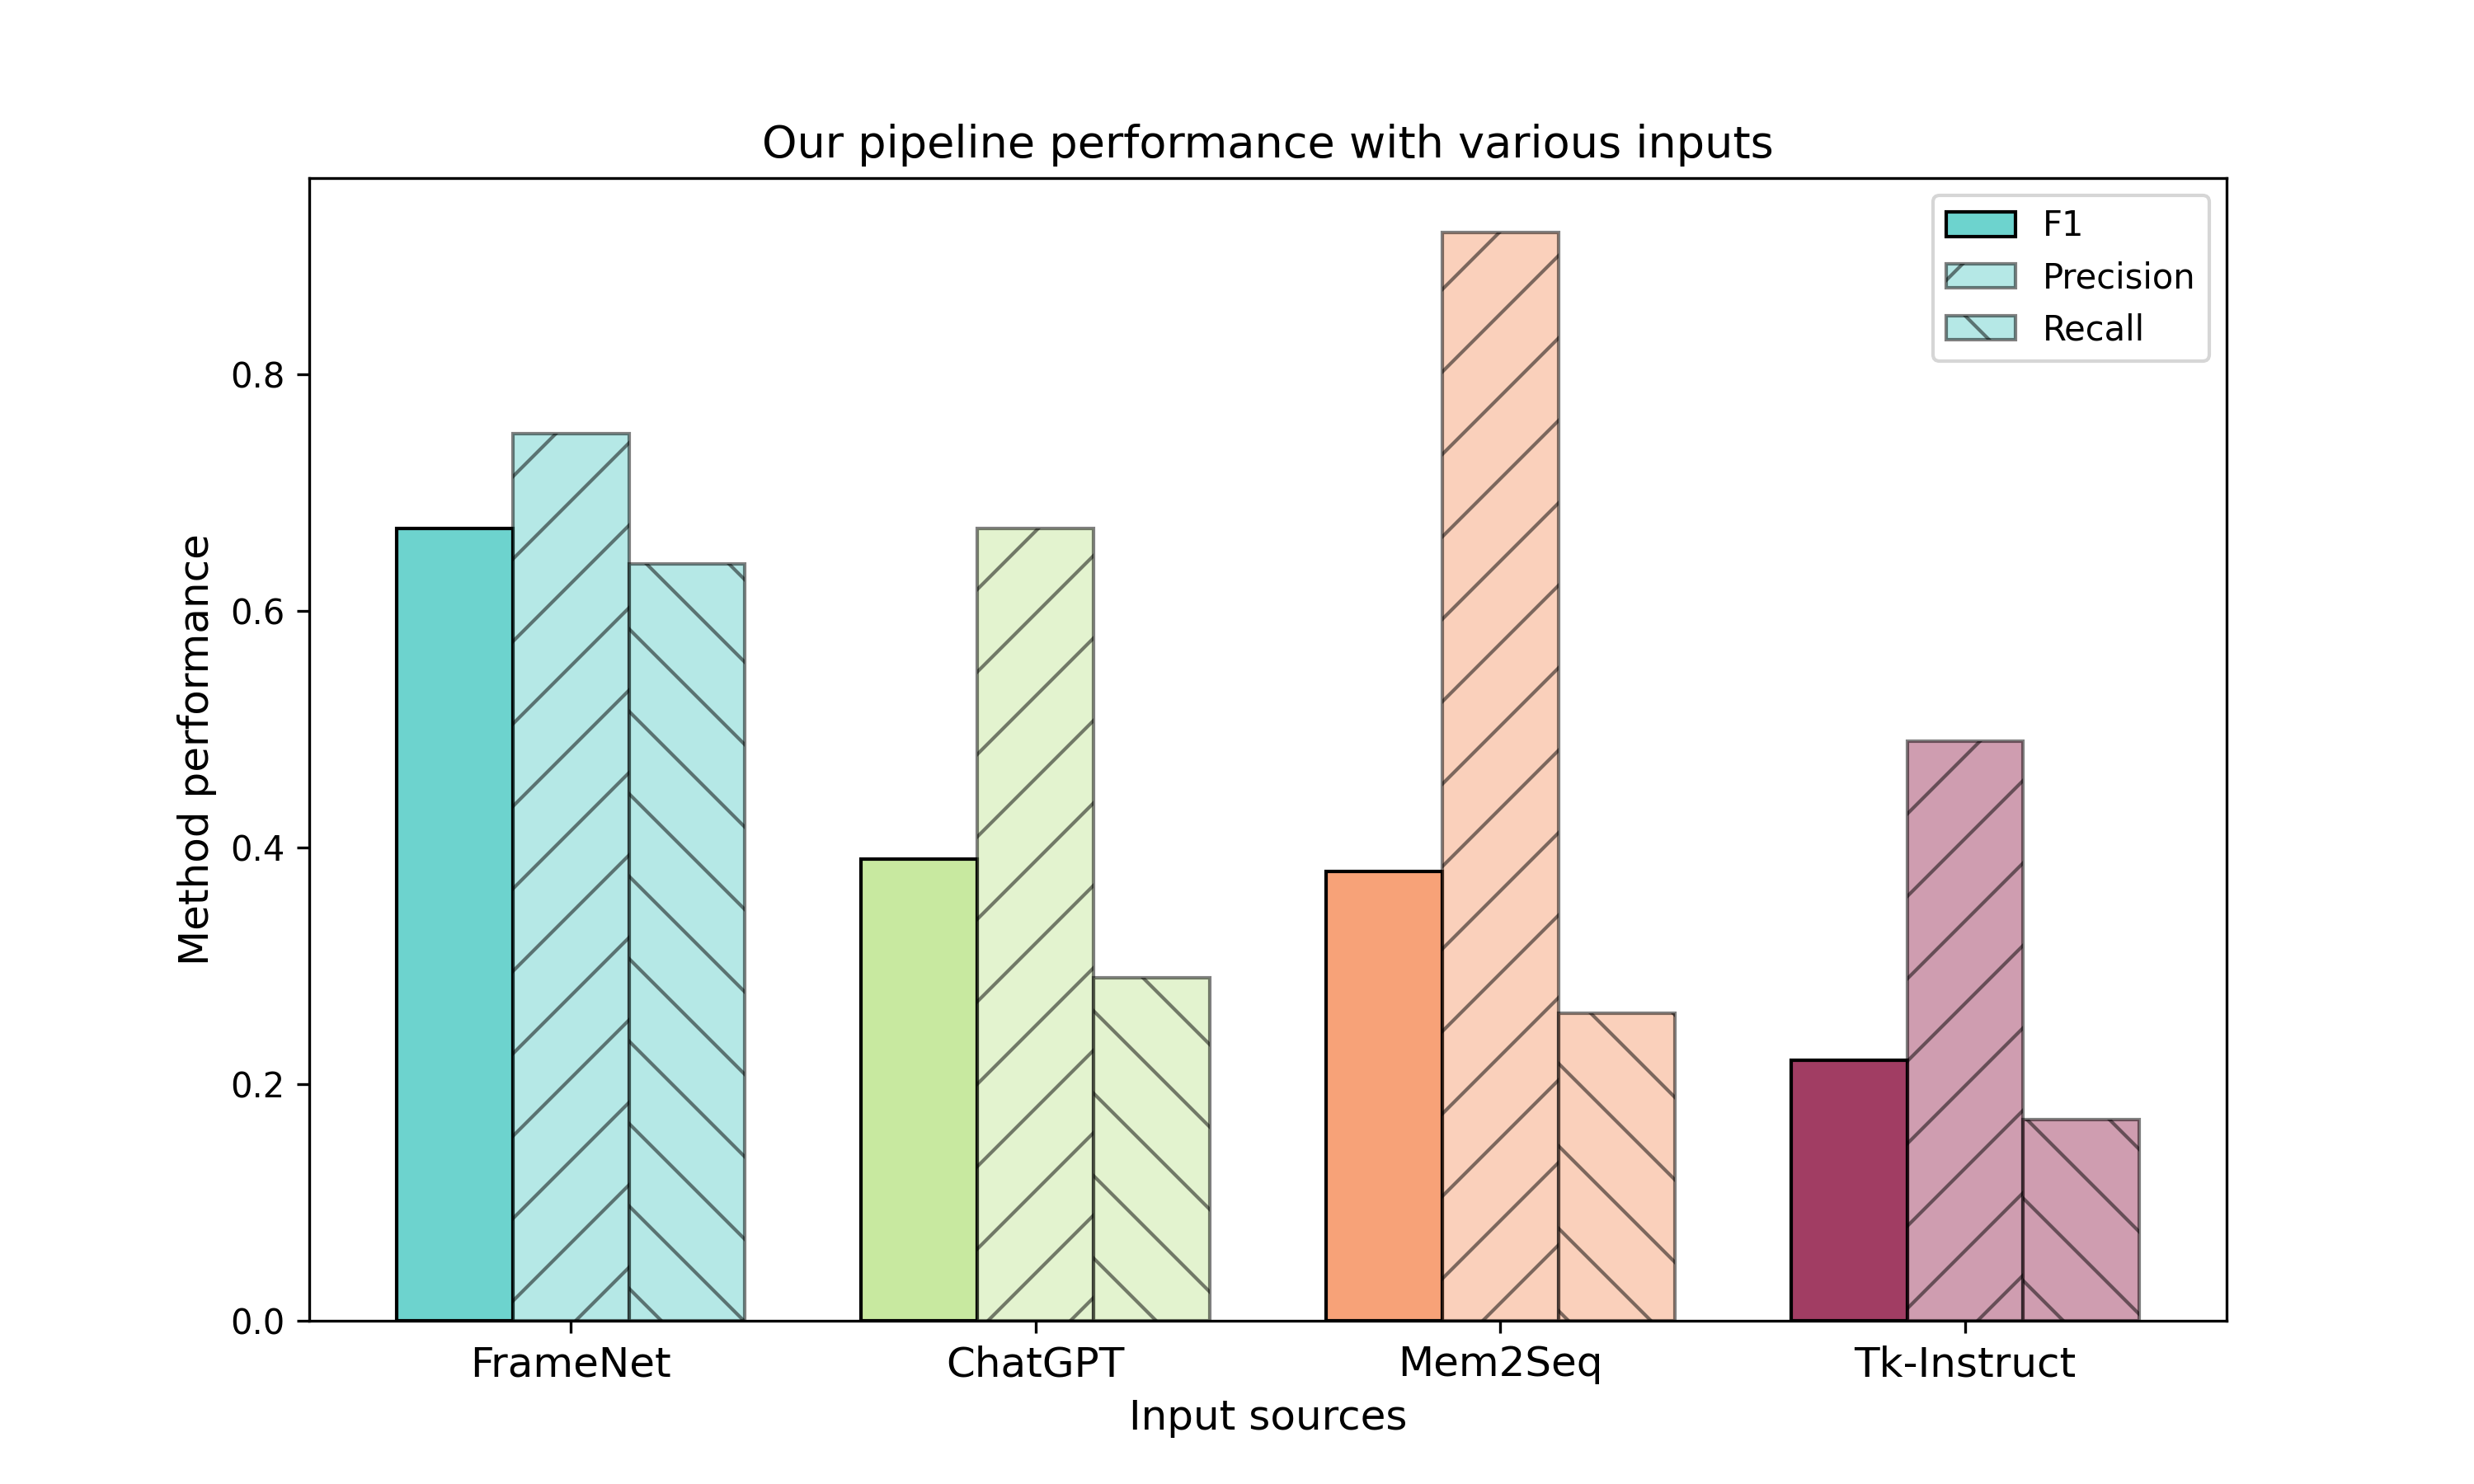
\includegraphics[width=0.9\textwidth]{images/slot-discovery.png}
    \caption{Comparison of our pipeline performance with different input sources. Note that FrameNet achieves both the best performance and the best trade-off between Precision and Recall}
    \label{04:fig:compare_sources}
\end{figure}

\begin{table}[tp]
    \centering
    \small
    \begin{tabular}{lccc}
    \hline
     \textbf{method} & \textbf{Precision} & \textbf{Recall} & \textbf{F1} \\
     \hline
     Mem2Seq & 0.72 & 0.22 & 0.31 \\
     LLM-ChatGPT & 0.76 & 0.23 & 0.35 \\
     LLM-Tk-instruct & 0.78 & 0.08 & 0.14 \\
     Mem2Seq+Ours & 0.92 & 0.26 & 0.38 \\
     LLM-ChatGPT+Ours & 0.67 & 0.29 & 0.39 \\
     LLM-Tk-instruct+Ours & 0.49 & 0.17 & 0.22 \\
     
     \hline
    \end{tabular}
    
    \caption{Cluster assignment accuracy of our methods if we interpret the clustering as user intent detection. \textit{Majority} is a majority baseline, and \textit{Embedding} refers to an average sentence embedding clustering approach.
    }
    \label{04:tab:unsup-discovery}
\end{table}


\subsection{Error analysis}
We conducted a manual error analysis of slot tagging to gain more insight into the output quality and sources of errors.
We found that the tagger can generalize and capture unseen values.

One source of errors is the relatively low recall of the frame-semantic parsers.
We successfully addressed this issue by introducing the slot tagger.
However, many slot values remain untagged.
This is expected as the input linguistic annotation quality inherently limits our method's performance.
The candidate merging procedure causes another error (see also below).
Due to frequent co-occurrence, two semantically unrelated candidates might be merged, and therefore, some tokens are wrongly included as respective slot fillers.
Nevertheless, the merging step is required to obtain a reasonable number of slots for a dialogue domain.

Our approach does leave some room for improvements, especially regarding the consistency of results across different slots, which can be imbalanced.
\begin{table}[tp]
    \centering
    \small
    \begin{tabular}{l|ccccccccc}
    \hline
    \textbf{dataset} & \textbf{price} & \textbf{area} & \textbf{request} & \textbf{type} & \textbf{food} & \textbf{day} & \textbf{people} & \textbf{stars} & \textbf{stay}
    \\ \hline
    \textbf{CR} & 0.54 & 0.76 & 0.76 & -- & 0.59 & -- & -- & -- & -- \\
    \textbf{CS} & 0.63 & 0.84 & 0.48 & 0.81 & 0.64 & -- & -- & -- & -- \\
    \textbf{WH} & 0.21 & 0.52 & 0.11 & 0.13 & -- & 0.15 & 0.82 & 0.82 & 0.34 \\
    \hline
    \end{tabular}
    
    \caption{Per-slot F1 scores of the \emph{Ours-full} method evaluated on selected datasets with slot intersection. For some slots, the performance varies a lot among datasets due to different ranges of values and contexts. The measures are evaluated using a manually designed slot mapping to the datasets' annotation, which is unnecessary for the methods.}
    \label{table:slotfilling_detail}
\end{table}

\paragraph{Slot candidate ranking}\hspace{-3mm} results are given in Table~\ref{table:avg-precision}.
Our pipeline significantly outperforms \citet{chen2014leveraging}'s approach on 4 out of 5 datasets.
We can also see that the slot-verb pairs clustering step is important -- in the ablation experiment where we do not perform clustering (\emph{Ours-nocl}),
performance falls dramatically on the WOZ-hotel, WOZ-attr, and ATIS data.
This is because, without the clustering step, many context-irrelevant slot candidates are considered, hurting performance.

In addition, we include a detailed evaluation of the contribution of the individual slot candidate ranking scores.
Results in Table~\ref{table:ablation-ranking} suggest that all of our proposed scores improve the performance.
\begin{table}[tp]
    \centering
    \small
    \begin{tabular}{lccccc}
    \hline
    %\textbf{method} 
    \textbf{method} & \textbf{CR} & \textbf{CS} & \textbf{WH} & \textbf{WA} & \textbf{AT} \\
    \hline
    \multirow{2}{*}{Chen et al.} & $0.315$ & $0.272$ & $0.269$ & $0.393$ & $\pmb{0.267}$ \\
    & $\pm .002$ & $\pm .001$ & $ \pm .001$ & $ \pm .002$ & $ \pm .003$ \\ 
    \multirow{2}{*}{Ours-nocl} & $\pmb{0.519}$ & $0.376$ & $0.069$ & $0.176$ & $0.069$ \\
    & $\pm .003$ & $ \pm .003$ & $ \pm .074$ & $ \pm .016$ & $ \pm .008$ \\
    \multirow{2}{*}{Ours-full} & $\pmb{0.520}$ & $\pmb{0.400}$ & $\pmb{0.317}$ & $\pmb{0.403}$ & $0.208$ \\
    & $\pm .004$ & $\pm .003$ & $\pm .008$ & $ \pm .006$ & $ \pm .018$ \\

\hline
    \end{tabular}
    
    \caption{Slot candidate ranking average precision for all datasets}
    \label{table:avg-precision}
\end{table}
\begin{table}[tp]
    \centering
    \small
    \begin{tabular}{lc}
    \hline
     \textbf{configuration} & \bf F1 score\\
     \hline
     Ours-full & $\mathbf{0.663} \pm 0.012$ \\
     %\hline
     Ours -frq & $0.600 \pm 0.008$ \\
     Ours -coh & $0.582 \pm 0.012$ \\
     Ours -TextRank & $0.514 \pm 0.006$ \\

     %\hline
     \hline
    \end{tabular}
    \caption{Ablation study of slot ranking features on CamRest676. The full model is compared to variants left out of the scores.}
    \label{table:ablation-ranking}
\end{table}

\paragraph{Slot merging}\hspace{-3mm} evaluation is shown in Table~\ref{table:merging}.
Although candidates in the CamRest676 data are merged into slots reasonably well, other datasets show a relatively low performance.
The low RI scores result from errors in candidate ranking, which wrongly assigned high ranks to some rare, irrelevant candidates.
These candidates do not appear in the reference mapping and are assumed to form singular “pseudo-slots”.
However, they are typically joined with similar candidates in the merging process.
This leads to many pairs of candidates merged into one slot by our approach but appearing separately in the reference mapping.
Nevertheless, this behavior barely influences slot tagging performance as the candidates are rare.
\begin{table}[tp]
    \centering
    \small
    
    \begin{tabular}{ll|ccccc}
    \hline
      & \textbf{method}\hspace{-3mm} & \textbf{CR} & \textbf{CS} & \textbf{WH} & \textbf{WA} & \textbf{AT} \\
     \hline
     \multirow{2}{*}{\textbf{RI}} & Rnd & $0.466$ & $0.268$ & $0.155$ & $0.153$ & $0.178$ \\
     & Ours & $0.587$ & $0.319$ & $0.168$ & $0.188$ & $0.171$ \\\hline
     \multirow{2}{*}{\textbf{NMI}\hspace{-2mm}} & Rnd & $0.212$ & $0.137$ & $0.061$ & $0.128$ & $0.171$ \\
     & Ours & $0.359$ & $0.207$ & $0.101$ & $0.117$ & $0.194$ \\

     \hline
    \end{tabular}
    
    \caption{Slot merging evaluation using RI and NMI on selected datasets, comparing our approach (\emph{Ours}) with a random baseline (\emph{Rnd}).}
    \label{table:merging}
\end{table}

\paragraph{Clustering evaluation:} 
Table \ref{table:intentclust} suggests that our clustering performs better than simple baselines and can yield useful results for intent detection.
Nevertheless, intent detection is more complex and presumably requires more features and information about the dialogue context, which we reserve for future work.
The complexity is also suggested by the naive embedding clustering performing worse than the majority baseline in 4 out of 5 cases.
\begin{table}[tp]
    \centering
    \small
    \begin{tabular}{lccccc}
    \hline
     \textbf{method} & \textbf{CR} & \textbf{CS} & \textbf{WH} & \textbf{WA} & \textbf{AT} \\
     \hline
     Majority & $0.592$ & $0.530$ & $0.883$ & $0.612$ & $\pmb{0.727}$ \\
     Embedding & $0.535$ & $0.551$ & $0.873$ & $0.595$ & $0.705$ \\
     Ours & $\pmb{0.705}$ & $\pmb{0.613}$ & $\pmb{0.882}$ & $\pmb{0.699}$ & $0.677$ \\
     \hline
    \end{tabular}
    
    \caption{Cluster assignment accuracy of our methods if we interpret the clustering as user intent detection. \textit{Majority} is a majority baseline, and \textit{Embedding} refers to an average sentence embedding clustering approach.
    }
    \label{table:intentclust}
\end{table}


% \subsection{Slot tagging precision and recall}
% \label{sec:app-pr}
% \begin{table}[tp][h]
%         \centering
%         \small
%         \begin{tabular}{l|cc|cc|cc|cc|cc|cc}
%          \hline
%           \multirow{2}{*}{\textbf{method}} & \multicolumn{2}{c|}{\textbf{CR}} & \multicolumn{2}{c|}{\textbf{CS}} & \multicolumn{2}{c|}{\textbf{WH}} & \multicolumn{2}{c|}{\textbf{WA}} & \multicolumn{2}{c}{\textbf{AT}} & \multicolumn{2}{c}{\textbf{AT(+NER)}} \\
%          %\hline
%            & P & R & P & R & P & R & P & R & P & R & P & R \\
%         \hline
%         Tag-supervised$^\ast$\hspace{-2mm} & $0.794$ & $0.814$ & $0.823$ & $0.696$ & $0.880$ & $0.683$ & $0.802$ & $0.715$ & $0.772$ & $0.913$ & -- & -- \\
%         Dict-supervised$^\ast$\hspace{-2mm} & $0.793$ & $0.710$ & $0.831$ & $0.752$ & $0.869$ & $0.710$ & $0.669$ & $0.859$ & $0.546$ & $0.990$ & -- & -- \\
%         \hline
%          Chen et al. & $\textbf{0.771}$  & $0.486$ & $\textbf{0.813}$ & $0.529$ & $0.384$ & $0.579$ & $0.362$ & $0.462$ & $0.701$ & $0.583$ & -- & --
%          \\\hdashline[0.5pt/2pt]
%          %\hline
%          Ours-nocl & $0.537$ & $0.347$ & $0.616$ & $0.371$ & $0.101$ & $0.218$ & $0.244$ & $0.340$ & $0.634$ & $0.595$ & $0.662$ & $0.704$ \\
%          %\hline
%          Ours-notag & $0.561$ &  $0.586$ & $0.690$ & $0.688$ & $0.369$ & $0.607$ & $0.335$ & $0.575$ & $0.715$ & $0.642$ & $0.685$ & $0.623$  \\
%          Ours-nothr & $0.636$ & $0.549$ & $0.585$ & $0.566$ & $0.458$ & $0.575$ & $\textbf{0.394}$ & $0.561$ & $0.701$ & $0.687$ & $\textbf{0.710}$ & $0.697$ \\
%          %\hline
%          Ours-full & $0.752$ & $\textbf{0.643}$ & $0.718$ & $\textbf{0.703}$ & $\textbf{0.494}$ & $\textbf{0.750}$ & $0.373$ & $\textbf{0.606}$ & $0.684$ & $0.672$ & $0.703$ & $\textbf{0.725}$ \\
%          \hline
%         \end{tabular}
                 
%         \caption{Precision (P) and recall (R) values slot tagging performance comparison among different methods (see Section~\ref{sec:setups}; frames are used as weak supervision in all setups, the rightmost column on ATIS additionally uses NER). We can see consistent recall improvement when using our slot tagger. The measures are evaluated using a manually designed slot mapping to the datasets' annotation, which is not needed for the methods themselves (see Section~\ref{lbl:mapping}). $^\ast$Note that supervised setups are not directly comparable to our approach.
%         \label{table:slotfilling_pr}
%         }
% \end{table}

\section{Dialogue generation application}
To verify the usefulness of the labels discovered by our method, we use them to train and evaluate an end-to-end task-oriented dialogue system.
We choose Sequicity \cite{lei2018sequicity} based architecture for our experiments, an LSTM-based encoder-decoder model that uses a system of copy nets and two-stage decoding.
First, it decodes the dialogue state so the database can be queried externally.
Sequicity generates the system response conditioned on the belief state and database results in the subsequent step.
This architecture works with a flat representation of the dialogue state, i.e. the state is represented as a sequence of tokens -- slot values.

The basic architecture is further extended by \citet{jin2018explicit}.
They propose to model the dialogue state explicitly in a semi-supervised way.
They extend the end-to-end encoder-decoder dialogue response generation model of \citet{lei2018sequicity} by introducing an additional decoder with access to posterior information about the system response.
This allows them to train a state representation with a reconstruction loss on unsupervised examples, using the state as a limited memory for essential concepts (roughly corresponding to slots).
Their method can be applied fully unsupervised, but it still requires some in-domain annotations to achieve good performance.
The default Sequicity model uses gold-standard dialogue state annotation. However, a compatible state representation is directly obtainable from our labels simply by concatenating the labels aggregated in each turn from user utterances. Whenever a new value for a slot is found in user input by our tagger, it is either appended to the state representation or replaces a previous value of the same slot.

We run three versions of the \citet{jin2018explicit}'s model: \emph{Jin et al.\ supervised} is a model that is trained fully on supervised data to provide perspective on the achieved performance.
\emph{Jin et al.\ unsupervised} is, on the contrary, fully unsupervised, i.e. we provide no labeled examples during the training phase to give a fair comparison against our model.
Finally, \emph{Jin et al.\ weak-labels} does not use supervised labels but presents labels obtained by our method.

\begin{table}[tp]
    \centering
    \smaller
    \begin{tabular}{l|c|c|c}
    \hline
      \textbf{method} & \textbf{Slot F1} & \textbf{Joint Goal Accuracy} & \textbf{Entity Match Rate} \\
      %\hline
 %      & onto & no-onto & onto & no-onto & onto & no-onto \\
      \hline
        Jin et al.\ supervised & $0.967 \pm .001$ & $0.897 \pm .002$ & $0.869 \pm .004$ \\
        Jin et al.\ unsupervised & $0.719 \pm .002$ & $0.385 \pm .003$ & $0.019 \pm .002$ \\
        Jin et al.\ weak-labels & $0.709 \pm .011$ & $0.335 \pm .008$ & $0.269 \pm .012$ \\\hdashline[0.5pt/2pt]
        Ours-full (unsupervised) & $\pmb{0.756} \pm .004$ & $\pmb{0.465} \pm .007$ & $\pmb{0.368} \pm .008$ \\
     \hline
    \end{tabular}
    \caption{Evaluation on the downstream task of dialogue generation on CamRest676 data. We evaluate with respect to three state tracking metrics. The best results in an unsupervised setting are presented in bold.}
    \label{table:downstream}
\end{table}
\footnotetext{We present results taken in an unsupervised setting, i.e. when no ontology is available.}

\subsection{Results} We explore the influence that our labels have on sequence-to-sequence dialogue response generation in an experiment on the CamRest676 data (see Table~\ref{table:downstream}).
We can see that our method provides helpful slot labels that improve dialogue state tracking performance.
Our approach significantly improves all metrics compared to \citet{jin2018explicit}'s system used in a fully unsupervised setting.
We achieve better results than \citet{jin2018explicit}'s system, especially regarding entity match rate, suggesting that our model can provide consistent labels throughout the dialogue.
To make a fair comparison, we further evaluate \citet{jin2018explicit}'s system in a setting where it can learn from the labels provided directly by weak supervision (i.e., the frame-semantic parser, not filtered by our pipeline).
We observe an improvement in entity match rate, but it does not match the improvement achieved with our filtered labels. Surprisingly, slot F1 and joint goal accuracy even decreased slightly, 
which suggests that label quality is important and the noisy labels obtained directly from weak supervision are not useful enough.

\section{Conclusion}
In this chapter, we propose a pipeline method that analyzes a set of clusters of semantically related values and yields a set of candidates for dialogue slots relevant to the given task.
The methods can take unstructured conversation data as inputs and require no data labels as inputs.

We show that our pipeline can work with various candidate identification methods and improve their performance regardless of the particular setup.
The method also compares favorably to similar proposed approaches.

The analysis shows that our method is rather sensitive to the quality of input clusters, i.e. the input source performance.
Our method is easy to apply and has reasonable performance that improves with the quality of provided input slot candidates.

For future work in this area, we can consider applying better methods for text representations and parsing, which would likely improve the qualitative performance.
It is also desirable to address the need for setting empirical thresholds, especially in the slot candidate selection and merging phase, exploiting the power of pre-trained language models.
Overall, the method is model-agnostic in the sense that various components of the pipeline can be swapped with better-performing models, which would likely improve the quantitative performance.